%\chapter{Milestone 6}
\section{Milestone 6}
\begin{comment}
- not sure if correct 
- will need to discuss this
- kinda still goes up exponentially (beginning)
- no idea about those bumps could be because of bad code
- hella instable in general -> likes to explode
- explosion looks cool thou 
\end{comment}
\begin{figure}[!h]
	\begin{center}
		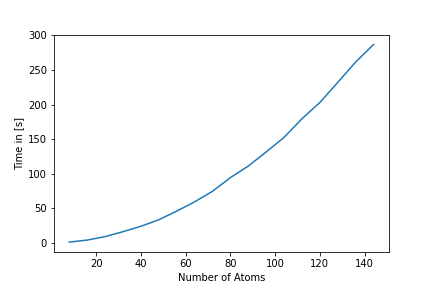
\includegraphics[scale=1]{Figure/plotAtomTimes.png}
	\end{center}
	\caption[Simulationtime without Neighborlist]{Simulationtime without Neighborlist}
	\label{PlotAtomTimesSecond}
\end{figure}
\begin{figure}[!h]
	\begin{center}
		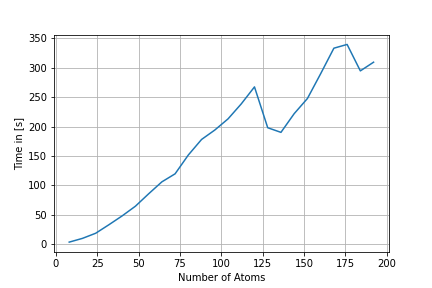
\includegraphics[scale=1]{Figure/plotAtomTimesTree.png}
	\end{center}
	\caption[Simulationtime with the old Neighborlist]{Simulationtime with the old Neighborlist}
	\label{PlotAtomTimesOldNeighbor}
\end{figure}

\begin{figure}[!h]
	\begin{center}
		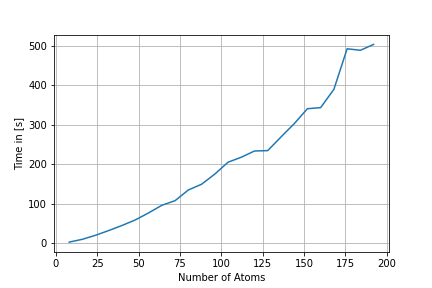
\includegraphics[scale=1]{Figure/plotAtomTimesNew.png}
	\end{center}
	\caption[Simulationtime with the new Neighborlist]{Simulationtime with the new Neighborlist  }
	\label{PlotAtomTimesCutoff}
\end{figure}